%%%%%%%%%%%%%%%%%%%%%%%%%%%%%%%%%%%%%%%%%%%%%%%%%%%%%%%%%%%%%%%%%%%%%%%%%%%%%%%%
%2345678901234567890123456789012345678901234567890123456789012345678901234567890
%        1         2         3         4         5         6         7         8
\documentclass[draftclsnofoot, onecolumn]{IEEEtran}
% \documentclass[letterpaper, 10 pt, conference]{ieeeconf}  % Comment this line out if you need a4paper
% \documentclass[a4paper, 10pt, conference]{ieeeconf}      % Use this line for a4 paper
\usepackage{color}
\usepackage[utf8]{inputenc}
\usepackage{graphicx}
\usepackage{wrapfig}
\usepackage{calc,cite}
\usepackage{textcomp}
\usepackage{url}
\usepackage{amsmath,multirow}
\usepackage{amssymb,float}
\usepackage{algorithm, algpseudocode}
\PassOptionsToPackage{normalem}{ulem}
\usepackage{ulem}
\renewcommand{\nu}{\ensuremath{\mathbf{n}(\mathbf{u})}\xspace}  % the normal vector at pixel location \V{u}
\newcommand{\pu}{\ensuremath{\mathbf{p}(\mathbf{u})}\xspace}   % the 3d point correspoinding the pixel \V{u}
\newcommand{\du}{\ensuremath{d(\mathbf{u})}\xspace}  
\newcommand{\zu}{\ensuremath{z(\mathbf{u})}\xspace}
\newcommand{\eu}{\ensuremath{\mathbf{e}(\mathbf{u})}\xspace}
\newcommand{\up}{\ensuremath{\V{u}_{\V{p}}}\xspace}
\newcommand{\tup}{\ensuremath{\tilde{\V{u}}_{\V{p}}}\xspace}

\newcommand{\oz}{\ensuremath{\Omega_z}\xspace}  
\newcommand{\on}{\ensuremath{\Omega_n}\xspace}
\newcommand{\Nu}{\ensuremath{\mathcal{N}(\V{u})}\xspace}

\renewcommand{\ni}{normal integration\xspace}
\newcommand{\NI}{Normal Integration\xspace}
\newcommand{\dpe}{discrete Poisson's equation\xspace}
\newcommand{\Dpe}{Discrete Poisson's equation\xspace}


\newcommand{\z}{\ensuremath{\V{z}}\xspace}
\newcommand{\zs}{\ensuremath{\V{z}^*}\xspace}
\newcommand{\rz}{\ensuremath{\red{\V{z}}}\xspace}
\newcommand{\zt}{\ensuremath{\V{z}_{t}}\xspace}
\newcommand{\zto}{\ensuremath{\V{z}_{t+1}}\xspace}
\newcommand{\R}{\ensuremath{\mathbb{R}}\xspace}
\newcommand{\fz}{\ensuremath{f(\V{z})}\xspace}

\newcommand{\rt}{\ensuremath{\V{r}_{t}}\xspace}
\newcommand{\rto}{\ensuremath{\V{r}_{t+1}}\xspace}


\newcommand{\dup}{\ensuremath{\V{D}_u^{+}}\xspace}
\newcommand{\dun}{\ensuremath{\V{D}_u^{-}}\xspace}
\newcommand{\dvp}{\ensuremath{\V{D}_v^{+}}\xspace}
\newcommand{\dvn}{\ensuremath{\V{D}_v^{-}}\xspace}
\newcommand{\nx}{\ensuremath{\V{n}_x}\xspace}
\newcommand{\ny}{\ensuremath{\V{n}_y}\xspace}
\newcommand{\nz}{\ensuremath{\V{n}_z}\xspace}
\newcommand{\Nz}{\ensuremath{\V{N}_z}\xspace}

\newcommand{\ft}{\ensuremath{F(\red{\V{z}};\V{z}_t)}\xspace}
\newcommand{\ftt}{\ensuremath{F(\V{z}_t;\V{z}_t)}\xspace}
\newcommand{\fto}{\ensuremath{F(\V{z}_{t+1};\V{z}_t)}\xspace}

\newcommand{\dpu}{\ensuremath{\partial_u \V{p}}\xspace}
\newcommand{\dpv}{\ensuremath{\partial_v \V{p}}\xspace}

\renewcommand{\u}{\ensuremath{\V{u}}\xspace}
\newcommand{\dzdu}{\ensuremath{\partial_u z}\xspace}
\newcommand{\dzdv}{\ensuremath{\partial_v z}\xspace}
\newcommand{\dztdu}{\ensuremath{\partial_u \tilde{z}}\xspace}
\newcommand{\dztdv}{\ensuremath{\partial_v \tilde{z}}\xspace}
\newcommand{\dzpdu}{\ensuremath{\partial_{u}^{+} z}\xspace}
\newcommand{\dzpdv}{\ensuremath{\partial_{v}^{+} z}\xspace}
\newcommand{\dzndu}{\ensuremath{\partial_{u}^{-} z}\xspace}
\newcommand{\dzndv}{\ensuremath{\partial_{v}^{-} z}\xspace}

\newcommand{\dzpduv}{\ensuremath{\partial_{\{u,v\}}^{+} z}\xspace}
\newcommand{\dznduv}{\ensuremath{\partial_{\{u,v\}}^{-} z}\xspace}
\newcommand{\dzduv}{\ensuremath{\partial_{\{u,v\}} z}\xspace}

\newcommand{\dupz}{\ensuremath{\Delta_{u}^{+} z}\xspace}
\newcommand{\dunz}{\ensuremath{\Delta_{u}^{-} z}\xspace}
\newcommand{\dvpz}{\ensuremath{\Delta_{v}^{+} z}\xspace}
\newcommand{\dvnz}{\ensuremath{\Delta_{v}^{-} z}\xspace}

\newcommand{\nuv}{\ensuremath{\V{n}(u,v)}\xspace}
\newcommand{\zuv}{\ensuremath{z(u,v)}\xspace}
\newcommand{\puv}{\ensuremath{\V{p}(u,v)}\xspace}

\newcommand{\halfpi}{\ensuremath{\pm {\pi \over 2}}\xspace}


\newcommand{\curve}{\ensuremath{\mathbb{S}}\xspace}
\newcommand{\zenith}{zenith\xspace}
\newcommand{\surface}{\ensuremath{\mathcal{M}}\xspace}
\newcommand{\visibility}{\ensuremath{\Phi_{i}}\xspace}
\newcommand{\point}{\ensuremath{\V{x}}\xspace}
\newcommand{\normal}{\ensuremath{\V{n}}\xspace}
\newcommand{\tangent}{\ensuremath{\V{t}}\xspace}
\newcommand{\cameraNum}{\ensuremath{C}\xspace}
\newcommand{\cameraCenter}{\ensuremath{\V{o}_{i}}\xspace}
\newcommand{\viewDirection}{\ensuremath{\V{v}}\xspace}
\newcommand{\batchsize}{\ensuremath{P}\xspace}
\newcommand{\mask}{\ensuremath{O}\xspace}
\newcommand{\projectedTangentVector}{projected tangent vector\xspace}
\newcommand{\projectedTangentVectors}{projected tangent vectors\xspace}
\newcommand{\stackedTangentVectors}{\ensuremath{\V{T}(\point)}\xspace}
\newcommand{\diligentmv}{\mbox{DiLiGenT-MV}\xspace}
\newcommand{\diligent}{DiLiGenT}
\newcommand{\loss}{\mathcal{L}\xspace}
\newcommand{\opticalAxis}{\ensuremath{\V{e}_{z}\xspace}}
\newcommand{\opticalAxisViewI}{\ensuremath{\V{e}_{z_{i}}}\xspace}
\newcommand{\opticalAxisMatrix}{\ensuremath{\V{C}}\xspace}
\newcommand{\ms}{Mumford-Shah integrator\xspace}
\newcommand{\made}{MADE\xspace}

\newcommand{\pandora}{\mbox{PANDORA}\xspace}
\newcommand{\psnerf}{\mbox{PS-NeRF}\xspace}
\newcommand{\sdps}{\mbox{SDPS}\xspace}
\newcommand{\uanet}{\mbox{UA-MVPS}\xspace}
\newcommand{\rmvps}{\mbox{R-MVPS}\xspace}
\newcommand{\bmvps}{\mbox{B-MVPS}\xspace}
\newcommand{\volsdf}{\mbox{VolSDF}\xspace}
\newcommand{\unisurf}{\mbox{UNISURF}\xspace}


\newcommand{\mvas}{MVAS\xspace}

\newcommand{\tsc}{\mbox{TSC}\xspace}

\newcommand{\pointOne}{\ensuremath{\point_1}\xspace}
\newcommand{\pointTwo}{\ensuremath{\point_2}\xspace}
\newcommand{\pointsetOne}{\ensuremath{\chi_{1}}\xspace}
\newcommand{\pointsetTwo}{\ensuremath{\chi_{2}}\xspace}
\newcommand{\fscoreThreshold}{\ensuremath{\tau}\xspace}
\newcommand{\chamferDist}{\ensuremath{d(\pointsetOne, \pointsetTwo)}\xspace}
\newcommand{\precision}{\ensuremath{\mathcal{P}}\xspace}
\newcommand{\recall}{\ensuremath{\mathcal{R}}\xspace}
\newcommand{\fscore}{\ensuremath{\mathcal{F}}\xspace}

\newcommand{\phaseangle}{\ensuremath{\hat{\phi}}\xspace}
\newcommand{\azimuthangle}{\ensuremath{\phi}\xspace}

\newcommand{\colorbar}[3]{
\begin{tabular}[t]{@{}l@{}l@{}}
	\includegraphics[height=#1\linewidth,width=0.5em]{colorbar.pdf} & 
	\begin{tabular}[b]{@{}l}
		#2 \\ [#3pt]
		$0$
	\end{tabular}
\end{tabular}
}


% \usepackage{subfigure}
\usepackage{subcaption}
\usepackage{textcomp}
\usepackage{array,setspace,booktabs,multirow,enumitem}
\usepackage{tikz}
\usetikzlibrary{fit,positioning,calc}
\def\BibTeX{{\rm B\kern-.05em{\sc i\kern-.025em b}\kern-.08em
		T\kern-.1667em\lower.7ex\hbox{E}\kern-.125emX}}
\newcommand{\linebreakand}{%
  \end{@IEEEauthorhalign}
  \hfill\mbox{}\par
  \mbox{}\hfill\begin{@IEEEauthorhalign}
} 
\makeatother
% This command is only needed if 
% you want to use the \thanks command
                                                         



\title{\LARGE \bf
Learning An Active Inference Model of Driver Perception and Control:
Application to Vehicle Car-Following}
%{\color{blue} an Active Inference} 
%Learning Interpretable models of Human Perception and Control: Applications to Vehicle Car-Following

\author{\IEEEauthorblockN{Ran Wei\IEEEauthorrefmark{1},
Alfredo Garcia \IEEEauthorrefmark{2},
Anthony D. McDonald \IEEEauthorrefmark{3}, \\
Gustav Markkula \IEEEauthorrefmark{3},
Johan Engstrom \IEEEauthorrefmark{4} and
\IEEEauthorrefmark{5} Matthew O'Kelly}
\\
\IEEEauthorblockA{\IEEEauthorrefmark{1} \IEEEauthorrefmark{2} Texas A\&M University}\\
\IEEEauthorblockA{\IEEEauthorrefmark{3}
University of Wisconsin}\\
\IEEEauthorblockA{\IEEEauthorrefmark{3} Leeds University}\\
\IEEEauthorblockA{\IEEEauthorrefmark{4} \IEEEauthorrefmark{5} Waymo}}





%\author{Ran Wei, Alfredo Garcia, A.D. McDonald, G. Markkula, J. Engstr{\"o}m and M. O'Kelly}



\begin{document}
\maketitle

\begin{abstract}
In this paper we introduce a general estimation methodology for learning a model of human perception and control in a sensorimotor control task based upon a finite set of demonstrations. 
The model's structure consists of {\em (i)} the agent’s internal representation of the world as the environment and associated observations
evolve as a result of control actions and {\em (ii)} the agent’s preferences over observable
outcomes. We consider a model's structure specification consistent with {\em active inference}, a theory of human perception and behavior from cognitive science.
According to active inference, the agent acts upon the world so as to minimize {\em surprise} defined as the sum of a measure of mismatch between {\em perceived} vs {\em preferred} states of the world and a measure of uncertainty in expected outcomes. We propose a bi-level optimization approach to estimation which relies on a structural assumption on prior distributions that parameterize the statistical accuracy of the human agent's model of the environment.
To illustrate the proposed methodology, we present the estimation of a model for
car-following behavior based upon a naturalistic dataset consisting of the positions, velocities, and headings of all vehicles in a road segment at a given sampling frequency. 
The results indicate that active inference-based model outperforms those obtained by imitation learning-based models from the machine learning literature and rule-based models commonly used in traffic simulation software. More importantly, 
the learned model exhibits better generalization performance on counterfactuals (i.e., predicting behavior with observation-action sequences not in the dataset).
Such
predicted behavior can be interpreted in terms of the agent's  categorical perception of risk in different states of the world and idiosyncratic preferences over features such as relative velocity and distance. Overall, the results indicate that learning active-inference models of human perception and control from data is a promising alternative to black-box models of driving.
\end{abstract}
 \IEEEpeerreviewmaketitle
 


\section{Introduction}
\label{intro}

 
In many control tasks requiring mind and motor resources by a human agent, the observation space can be high-dimensional and complex. Empirical evidence indicates that humans agents use a simpler, lower dimensional representation of the environment in sensorimotor control tasks \cite{Badre_2021, DeBeek_2002}. The Bayesian brain hypothesis \cite{Knill_2014, Friston_2012} posits that the human brain represents sensory information in the form of probability distributions over a lower dimensional representation of the environment. To account for the structure of human perception and control in a task involving motor and mind resources, a model must separately describe {\em (i)} the agent’s internal representation of the world as the environment
evolves as a result of control actions and {\em (ii)} the agent’s preferences over observable
outcomes. Equipped with data in the form of demonstrations (i.e. sequences of recorded observation-action pairs), the learning task is to estimate the agent’s preferences as well as its internal representations leading to a behavior policy that best fits data. 

In machine learning and artificial intelligence, this estimation problem is known as {\em inverse} reinforcement learning (IRL) in an {\em off-line} setting \cite{Osa_2018}.
The goal of IRL is to estimate the reward function and policy of a value-maximizing agent from its observed behavior \cite{ng2000algorithms, osa2018algorithmic,Abazar_2020}. The estimated reward has a number of use cases, including designing policies in domains where manual reward specification is difficult, e.g., in autonomous driving \cite{Phan_2023}, and obtaining novel insight about a target population and device interventions, such as in biology, economics, and human-robot interaction \cite{yamaguchi2018identification, Rust_1994, sadigh2018planning}.
There is a significant literature on the {\color{blue} identification and estimation of human control models} when the state is observable \cite{Boer_1998,Van_2016, Drop_2018}.
In contrast, {\color{blue} model identification and estimation} when the state is only partially observable (as in models accounting for human perception) has received less attention.
Notable exceptions include \cite{Baker_2017, Chang_2022, Straub_2022, Pekkanen_2018}. However, the environments considered in these papers are either low dimensional as in \cite{Baker_2017, Chang_2022},  restricted to a linear-quadratic control \cite{Straub_2022} or customized for a specific control task \cite{Pekkanen_2018}.

In this paper, we introduce a Bayesian estimation methodology for learning a model of perception and control in general control tasks in higher dimensional settings. We use the formalism of a Partially Observable Markov Decision Process (POMDP) in which the agent's preferences are modeled by a reward function and the agent's internal representation of the environment consists of observation and transition probabilities.
However, a POMDP model of a human agent's perception and control policy based solely on demonstrations is in general {\em non-identifiable}, i.e. there may be several different combinations of reward and internal model of the environment that rationalize the same demonstrations dataset. This is because in planning control tasks different combinations of reward and internal model dynamics could result in the same inter-temporal reward trade-offs.
To address this issue, we make a structural assumption on prior distributions that parameterize the statistical accuracy of the human agent's model of the environment.
Specifically, we assume
({\em i}) the agent's preferences and model of the environment are independent and ({\em ii}) the distribution of the model of the environment parameters concentrates on values with higher fit to the data (i.e. higher log-likelihood).
In words, this assumption restricts our estimation to agents with reasonably accurate models of the environment whose preferences over states of the world are not determined by their perception of the environment. This allows us to formulate the {\em Maximum A Posteriori} (MAP) estimator as the solution to a bi-level optimization problem. The upper-level problem is the maximization of the posterior distribution and the inner-level problem is the computation of optimal policy for the given reward {\em and} model of the environment. We approximate the solution to this bi-level optimization problem by a stochastic gradient algorithm with a nested policy optimization step.

To illustrate the proposed methodology, we consider an application to
highway driving  using a naturalistic dataset consisting of the positions, velocities, and headings of all vehicles in a road segment at a given sampling frequency. We specify the structure of the model in accordance to ``active inference" \cite{friston2010free, Parr_2022, Maisto},
a novel framework for modeling human perception and behavior in sensorimotor control tasks. Active inference is related to the Bayesian Brain hypothesis that posits prediction as the fundamental task of cognition \cite{Clark_2015, Hohwy_2015}, i.e. the brain minimizes prediction error by updating beliefs about the states of the world consistent with data. Active inference takes a conceptual leap from this view in that minimizing prediction error can also be attained by both updating beliefs and acting upon the world to approximately induce a preferred distribution of the states of the world. The active inference framework is summarized by a principle of {\em free energy minimization}: forward (action) and backward (belief) updating processes work in tandem to minimize ``surprise" with respect to a preferred belief distribution about the states of the world.

We compare the learned structural model of perception and action (with an active inference reward specification) with two baseline models based on Behavior Cloning (BC), a common machine learning approach to driving behavior modeling \cite{suo2021trafficsim, igl2022symphony, codevilla2019exploring, zhou2017recurrent}, and the Intelligent Driver Model (IDM), a rule-based model used by most traffic simulation software \cite{treiber2000congested, treiber2013microscopic, kesting2009agents}.
The results indicate that active inference-based model outperforms those obtained by imitation learning-based models from the machine learning literature. In addition, we show that the learned model based upon active inference is better equipped to estimate counterfactuals (i.e., predict behavior with observation-action sequences not in the dataset) and trace those behaviors back to perception and driver preferences. The results indicate that learning active-inference models from data is a promising alternative to black-box models of driving.

The structure of this paper is as follows. In section II, we start by describing a Partially Observable Markov Decision Process (POMDP) of perception and control. In section III, we describe the inverse estimation problem, i.e. based upon sequences of observations and implemented actions to estimate the primitives of the POMDP model (reward, partially observable state transition and observation probabilities). In section IV, we describe the specification of reward function based upon active inference, a novel framework for cognition and behavior.
In section V, we describe the application of the proposed estimation algorithm to obtain an active-inference model  for car-following behavior by human drivers. We compare the active inference model with Behavior Cloning (BC) and the Intelligent Driver Model (IDM). Finally, in section VI, we close with concluding remarks about the promise and challenges of learning perception \& control models based upon naturalistic datasets. 


\subsection{A Preview of The Results}
To motivate the reader, we now provide a preview of the estimation results for the car following task.
In Figure \ref{fig:obs_scatter_data} the data for relative velocity $\Delta v$, relative distance $d$, inverse of time-to-collision $\tau$ and  acceleration $a$ (in color code) is shown. To get a visual sense of model fit, in Figure \ref{fig:obs_scatter_policy}, we display the observed features in $200$ trajectories sampled from the learned control policy and model of the environment. The substantial overlap between Figures
\ref{fig:obs_scatter_data} and \ref{fig:obs_scatter_policy} indicates that the learned model of perception and control produces observed features that are similar to those in the data.


\begin{figure}[!htb]
\centering
    \begin{subfigure}[b]{0.22\linewidth}
    \includegraphics[height=0.45\textheight, width=1\linewidth, trim={0 4.5cm 0 0}, clip]{fig/scatter_vert_data.png}
    \caption{}
    \label{fig:obs_scatter_data}
    \end{subfigure}
    %
    \begin{subfigure}[b]{0.22\linewidth}
    \includegraphics[height=0.45\textheight, width=1\linewidth, trim={0 4.5cm 0 0}, clip]{fig/scatter_vert_policy.png}
    \caption{}
    \label{fig:obs_scatter_policy}
    \end{subfigure}
    %
    \begin{subfigure}[b]{0.22\linewidth}
    \includegraphics[height=0.45\textheight, width=1\linewidth, trim={0 4.5cm 0 0}, clip]{fig/scatter_vert_cluster.png}
    \caption{}
    \label{fig:obs_scatter_cluster}
    \end{subfigure}
    %
    \begin{subfigure}[b]{0.22\linewidth}
    \includegraphics[height=0.45\textheight, width=1\linewidth, trim={0 4.5cm 0 0}, clip]{fig/scatter_vert_preference.png}
    \caption{}
    \label{fig:obs_scatter_preference}
    \end{subfigure}
\caption{Visualizations of active inference model In panel (a), we plotted observations sampled from the dataset. In panels (b), (c), and (d) we sampled 200 points from the model's state conditioned observation distributions and plotted the sampled points for each pair of observation feature combinations. The points in each panel are colored by: (a)  accelerations from the dataset, (b) predicted accelerations upon observing the sampled signals from a uniform prior belief, (c) state assignments (d) log probabilities of the preference distribution.}
\label{fig:obs_scatter}
\end{figure}

Going beyond this basic modeling expectation, Figure \ref{fig:obs_scatter_cluster} shows the {\em categorical} nature of perception learned by our model---represented through color coding of observations for different states (i.e, sample observations are drawn from the generative model that describe the distribution of observation given a state of the world). The distribution shows that the hidden states largely corresponds to different levels of safe operation (e.g. magnitudes of relative velocity and relative distance). This is consistent with satisficing---a well established driving behavior \cite{Summala_2007}. Finally, in Figure \ref{fig:obs_scatter_preference} the relative preferences for {\em low} magnitude values of relative velocity and distance are described in terms of a {\em preferred} distribution over observations pairs $(\Delta v,d)$. The lighter colored observations (yellow and orange hues) are preferred to darker colored ones (purple hues). Thus, the model learns driver preferences for maintaining safe following distances.




\section{A POMDP Model of Perception and Control}
\label{Sec:Model}

We start by providing a description of a partially Observable Markov Decision Process (POMDP) of perception and control. This encompasses neuroscience modeling frameworks for human perception and action in sensorimotor tasks such as {\em active inference} \cite{friston2010free} and the {\em expected value of control} (EVC) \cite{Shenhav_2017}. 

In the POMDP framework (see Figure \ref{graphical}), the human agent maintains an {internal} model of the world (or representation) so that high-dimensional observations $o_t \in O\subset \mathbb{R}^n$ (sensory stimuli) are represented with a lower dimensional {\em hidden} state $s_t \in S \subset \mathbb{R}^m$ where $S$ is the state space and $m<<n$. 
If the hidden state is $s_t$ and $a_t \in A$ is implemented, the agent accrues a reward $r(s_t, a_t)$. The agent's internal representation includes state dynamics, i.e. a transition to a new state $s_{t+1}$ takes place with probability $\mathbb{T}(s_{t+1}|s_t,a_t)$ and a new observation $o_{t+1}$ is obtained with probability $\mathbb{O}(o_{t+1}|s_{t+1})$. 

After $t>0$ time periods, the observable history of observations and actions is denoted by 
$$h_t:=\{o_t,...,o_0, a_{t-1},...,a_0\}\in H_t \subset O^{t+1}\times A^t.$$ 
We consider randomized policies $\pi$ that are adapted to the history of the process, i.e. given history $h_t$ action $a \in A$ is implemented with probability $\pi(a|h_t) \in [0,1], a \in A$ and $\sum_{a \in A} \pi(a|h_t)=1$ for all $h_t \in H_t$.

In the POMDP model of perception and action, the human agent aims to maximize the expected value of discounted reward net of information processing costs:
\begin{equation}    
U_{\tau}(h_{\tau})\triangleq \sup_{\pi \in \Pi} \mathbb{E}\Big[ \sum_{t\geq \tau} \gamma^{t-\tau} [r(s_{t}, a_{t})-c(\pi(\cdot|h_t))]\Big]
\label{U}
\end{equation}
where $\gamma \in (0,1)$ is the discount factor, $\Pi$ is the set of randomized policies that are adapted to the history process and $c(\pi(\cdot|h_t))$ is the per-period {\em information processing cost}.
As human agents may differ in their ability to process task-relevant information or to attend to the task at hand \cite{tishby2011information, Ortega_2013,Matejka_2015,Fudenberg_2015, Hansen_2018}, the information processing cost models the fact that {\em low} entropy behavioral policies are consistent with {\em high} information processing effort or attention.

The combination of additive reward structure and Markovian dynamics allows for a recursive characterization of the optimal policy as follows:
\begin{align}
 U_{t}(h_t) &= \max_{\pi(\cdot|h_t)} \Bigg \{ \sum_{a_t}\sum_{s_t} r(s_t, a_t)b_{t}(s_t)\pi(a_t|h_t) -c(\pi(\cdot|h_t))
 + \gamma \sum_{o_{t+1}}\sum_{a_t} \mathbb{P}(o_{t+1}|h_t, a_t)\pi(a_t|h_t)  U_{t+1}(h_{t+1}) \Bigg \}. \label{model}  &
\end{align}

\begin{wrapfigure}{r}{0.5\textwidth}
\centering 

  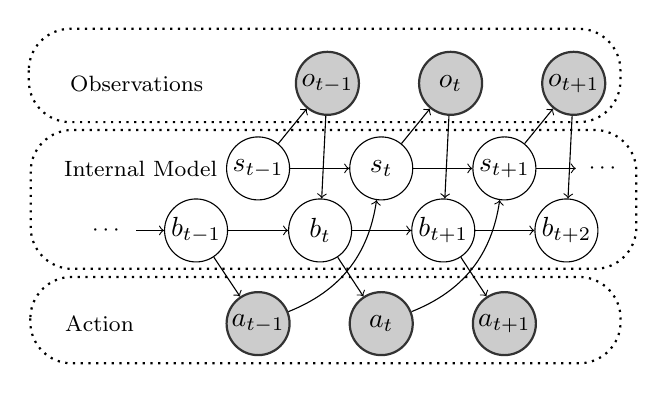
\begin{tikzpicture} 
    [node distance=12.5 pt and 24pt, every node/.style={draw, circle, inner sep=0pt}, minimum size=8mm]  

    
    \tikzstyle{obs}=[circle, draw, minimum size=8mm, thick, draw=black!80, fill=black!20, node distance=3mm] 
    \tikzstyle{label}=[rectangle, draw, minimum size=7mm, thick, draw=black!0, node distance=0mm] 

    \node [] (st) {\normalsize $s_t$};
    \node (s0) [left=0.75cm of st] {\normalsize $s_{t-1}$};
    \node [right=.75cm of st] (s1) {\normalsize $ s_{t+1}$};
    
    \node [obs, above right=.5cm and .3cm of st] (ot) {\normalsize $o_t$};
    \node [obs, above right=.5cm and .3cm of s0] (o0) {\normalsize $o_{t-1}$};
    \node [obs, above right=.5cm and .3cm of s1] (o1) {\normalsize $ o_{t+1}$}; 

    \node [below left=.3cm of s0] (b) {\normalsize $b_{t-1}$};  
    \node [below right=.3cm of s0] (b0) {\normalsize $b_{t}$};  
    \node [below right=.3cm of st] (bt) {\normalsize $b_{t+1}$};
    \node [below right=.3cm of s1] (b1) {\normalsize $b_{t+2}$};    
    
    \node [obs, below=1.15cm of s0] (a0) {\normalsize $a_{t-1}$};  
    \node [obs, below=1.15cm of st] (at) {\normalsize $ a_t$};  
    \node [obs, below=1.15cm of s1] (a1) {\normalsize $a_{t+1}$};
    \node[label,right = 0.5 cm of s1] (s2) {\footnotesize $\cdots$};
    \node[label,left = 0.35 cm of b] (b2) {\footnotesize $\cdots$};
    
    \path [->]
    (s0) edge (st)
    (b)  edge (b0)
    (b)  edge (a0)
    (st) edge (s1)
    (s0) edge (o0)
    (st) edge (ot)
    (s1) edge (o1)
    (o0) edge (b0)
    (ot) edge (bt)
    (o1) edge (b1)
    (b0) edge (bt)
    (bt) edge (b1)
    (b0) edge (at)
    (bt) edge (a1)
    (s1) edge (s2)
    (b2) edge (b);

     \path [->,draw] (at) edge[bend right] (s1);
    \path [->,draw] (a0) edge[bend right] (st);
    
    % add box 
    \draw[thick, dotted, rounded corners=15pt] ($(o0.north west)+(-3.5,.4)$)  rectangle ($(o1.south east)+(.3,-0.2)$);
    \node[label, left=of o0] [left = 1.15 cm of o0]{\footnotesize Observations};


    \draw[thick, dotted, rounded corners=15pt] ($(s0.north west)+(-2.6,0.2)$)  rectangle ($(b1.south east)+(0.6,-0.2)$);
    \node[label] [left= 0.10 cm of s0]{\footnotesize Internal Model};
    
    \draw[thick, dotted, rounded corners=15pt] ($(a0.north west)+(-2.6,0.3)$)  rectangle ($(b1.south east)+(0.4,-1.4)$);
    \node[label, left=of a0] [left = 1.15 cm of a0] {\footnotesize Action};
    \end{tikzpicture}%
\vspace{-0.10cm}
\caption{{\small Graphical Model of Perception and Control.}} 
\label{graphical}
\end{wrapfigure}




Let $b_{t} \in \Delta^S$ denote the Bayes updated belief distribution on the state, i.e. $b_{t}(s)=\mathbb{P}(s_t=s|h_t)$, where $\Delta^S$ is the simplex in $\mathbb{R}^m$.
Let us denote by $\sigma(o_{t+1}|b_{t},a_{t})$ the probability of recording observation $o_{t+1}$ when action $a_t$ is implemented and the current belief distribution is $b_t$, i.e.
\begin{align*}
\sigma(o_{t+1}|b_{t},a_{t}) &:=
\sum_{s_{t+1}}\sum_{s_t}\mathbb{O}(o_{t+1}|s_{t+1}) \mathbb{T}(s_{t+1}|s_t,a_t)b_{t}(s_t)
\end{align*}
Using standard POMDP arguments in Proposition 1 below we show that with no loss of optimality, the search for optimal policy can be restricted to {\em Markovian} policies, say $\Pi^M \subset \Pi$ that only depend $b_{t}$, the current Bayes updated belief as opposed to the whole history $h_t\in H_t$. 

\begin{proposition}
Let $V_{t}(b)$ be recursively defined as follows:
\begin{align*}
    &V_{t}(b) = \max_{\pi(\cdot|b)} \Big\{\sum_s\sum_{a} r(s, a)\pi(a|b)b(s) -c(\pi(\cdot|b)) + \gamma\sum_{a}\sum_{o'}\sigma(o'|b,a)\pi(a|b) V_{t+1}(b') \Big \}
\end{align*}
where $b'(s) =\mathbb{P}(s_{t+1}=s|h_t\cup(a,o'))$, i.e. the resulting Bayes update after action $a$ is implemented and observation $o'$ are recorded. Then, the Bayes updated belief $b_t=\mathbb{P}(\cdot|h_t)$ is a sufficient statistic for solving \eqref{model}, i.e. $U_{t}(h_t)=V_{t}(b_t)$ for all $h_t$.
\label{SufficientTheorem}
\end{proposition}
\begin{proof} See Appendix.
\end{proof}


We now state and prove the {\em soft} Bellman equation for the value function $V_t(b)$ when the information processing cost is proportional to the Kullback-Leibler divergence between the control policy and a default policy $\pi^{0}$, i.e. $c(\pi(\cdot|b_t)) =  
\alpha \mathcal{D}_{KL}(\pi(\cdot|b_t)||\pi^0(\cdot|b_t))$ where:
\begin{align}
 \mathcal{D}_{KL}(\pi(\cdot|b)||\pi^0(\cdot|b)) &:= \sum_{a \in A} \pi(a|b)\log \frac{\pi(a|b)}{\pi^0(a|b)}.
 \label{KL_divergence}
 \end{align} 
 and $\alpha>0$.


Let $\mathcal{Q}$ be the Banach space of bounded, measurable functions $Q: \Delta^S \rightarrow \mathbb{R}$ under the supremum norm $||.||$. Define the {\em soft} Bellman operator $\mathcal{B}: \mathcal{Q} \rightarrow \mathcal{Q}$ by 
\begin{align}
    [\mathcal{B}Q](b,a)&:= \sum_s r(s,a)b(s) + \gamma \sum_{o'}\sigma(o'|b, a)\alpha \log \Big(\sum_{a'}\pi^0(a'|b')\exp\big( \frac{1}{\alpha}Q(b',a')\big)\Big),
    \label{model4}
\end{align}
where $b'$ is the resulting Bayes update after action $a$ and observation $o'$ are recorded. 
\begin{theorem}
(a) $\mathcal{B}: \mathcal{Q}\rightarrow \mathcal{Q}$ is a contraction mapping with modulus $\gamma \in (0,1)$ with unique fixed point $Q^*$, (b)
\begin{align*}
V^*(b) & =\max_{\hat{\pi}(\cdot|b)}\Big[\sum_a \hat{\pi}(a|b)Q^*(b,a)-\alpha \mathcal{D}_{KL}\big(\hat{\pi}(\cdot|b)||\pi^0(\cdot|b)\big)\Big] \\
& =\alpha \log \sum_a \pi^0(a|b)\exp\big(\frac{1}{\alpha} Q^*(b,a)\big)
\end{align*}
(c) the optimal policy is of the form:
\begin{align}
  \pi^*(a|b)=\frac{\pi^0(a|b)\exp\big({\frac{1}{\alpha}Q^*(b,a)}\big)}{\sum_{a' \in A}\pi^0(a'|b)\exp\big({\frac{1}{\alpha}Q^*(b,a')}\big)}.  
\end{align}
\label{CCPTheorem}
\end{theorem}
\begin{proof} See Appendix. \end{proof}

\textbf{Remark 1}: Note that as $\alpha \rightarrow +\infty$, information processing effort is arbitrarily costly and in the limit, the agent implements the default policy $\pi^* \rightarrow \pi^0$. Conversely, as $\alpha \rightarrow 0^+$, we recover the optimal solution without information processing cost since $V^*(b) \rightarrow \max_{a\in A} Q^*(b,a)$.

\textbf{Remark 2}: In the remainder of the paper we shall use $\alpha=1$ and the default policy is the uniformly random policy $\pi^0(a|b)=\frac{1}{|A|}$. With these choices the optimal policy takes the form:
\begin{align}
  \pi^*(a|b)=\frac{\exp Q^*(b,a)}{\sum_{a' \in A}\exp Q^*(b,a')}.  
\end{align}

\textbf{Remark 3 (Finite Horizon)}: It can be easily verified that Proposition 1 and Theorem 1 continue to hold for the case in which the controller is solving a finite horizon problem. Evidently, the results in this case require that the state-action function $Q_{t}$ and the conditional choice probabilities $\pi_{t}$ are time-dependent $t$. Formally, for a planning horizon of length $H>0$, the optimal policy at time $t\in\{0,1,\dots, H\}$ is of the form:
\begin{align}
\pi_{t,H}^{*}(a|b&=\frac{\exp Q_{t,H}^{*}(b,a)}{\sum_{a' \in A}\exp Q_{t,H}^{*}(b,a')}
\label{receding_soft_policy}
\end{align}
and
\begin{align}
Q_{t,H}^*(b,a)&=\sum_s r(s,a)b(s) + \sum_{o'}
\sigma(o'|b, a)V^*_{t+1,H}(b')
\label{soft_optimal_value} 
\end{align}
where $b'$ is the resulting Bayes update after action $a$ and observation $o'$ are recorded and
\begin{align}
V^*_{t+1,H}(b') & =  \log \Big(\sum_{a'}\exp Q^*_{t+1,H}(b',a')\Big)~~~~t\leq H-1 \label{finite_horizon}
\end{align}
and $
V^*_{H+1,H}=0$.




\section{Estimation Methodology}
Equipped with a model of perception and action as described in the previous section, we consider the estimation of the primitives based upon demonstrations, that is, sequences of observations and implemented actions of the form $\tau = \{(o_1,a_0),(o_2,a_1),\dots,(o_{T+1},a_t)\}$. We shall denote by $\mathcal{D}$ the finite dataset of distinct sequences of observation-action pairs. 

The primitives of the perception \& control model are parametrized as follows:

\begin{itemize}
    \item 
{\em Perception} We assume the agent's internal representation of hidden state dynamics and observation probabilities is parametrized with $\theta_1 \in \mathbb{R}^p_1$ so that the likelihood of observation $o_{t+1}$ given beliefs $b_t$ and action $a_t$ is $ \sigma_{\theta_1}(o_{t+1}|b_{t},a_t)$.

\item {\em Preferences} A reward function $r_{\theta_2}(b,a)$ which is parametrized by $\theta_2 \in \mathbb{R}^p_2$. 
\end{itemize}

Assuming the data is generated by an agent who uses a {\em receding horizon} plan with horizon $H$ according to \eqref{receding_soft_policy}, the log-likelihood of a sequence $\tau \in \mathcal{D}$ can be written as
\begin{align*}
\mathbb{P}(\tau|\theta)&=  \prod_{t=0}^T\Big(\pi^{*}_{\theta}(a_{t}|b_{\theta_1,t})\mathbb{P}\big(o_{t+1}|h_{t} \cup 
\{a_t\}\big)\Big)
\end{align*}
where to alleviate notation we write $\pi^{*}_{\theta}(\cdot|b)$ to refer to the first-period optimal policy with a planning horizon $H>0$.
Hence, the log-likelihood of dataset $\mathcal{D}$ can be written as:
\begin{align}
\log \mathbb{P}(\mathcal{D}|\theta)&= \log \prod_{\tau \in \mathcal{D}} \mathbb{P}(\tau|\theta) \nonumber \\
&=\mathbb{E}_{\tau \sim \mathcal{D}}\Big[ \sum_{t=0}^T\log\Big(\pi^{*}_{\theta}(a_{t}|b_{\theta_1,t})\mathbb{P}\big(o_{t+1}|h_t \cup \{a_t\}\big)\Big)\Big]|\mathcal{D}| \\
&=\mathbb{E}_{\tau \sim \mathcal{D}}\Big[ \sum_{t=0}^T\log\pi^{*}_{\theta}(a_{t}|b_{\theta_1,t})\Big]|\mathcal{D}| + \mbox{constant} \label{likelihood}
\end{align}
where the expectation is taken with respect to the empirical measure $\bar{\mathbb{P}}(\tau)=\frac{1} {|\mathcal{D}|}$ and
\begin{align}
\pi_{\theta}^*(a|b)& =\frac{\exp{Q_{\theta}^{*}(b,a)}}{{\sum_{a' \in A} \exp {Q_{\theta}^{*}(b,a')}}} \label{softmax}
\end{align}
Condition \eqref{softmax} imposes model in the form of the first period policy of a receding horizon plan. 
% that minimizes total free energy. 

We take a Bayesian approach to finding an estimator and make an additional assumption on the structure of the prior distribution of parameters denoted by $P(\theta)$: 

{\bf Assumption 1}:
(a) $P(\theta) = P(\theta_1)P(\theta_2)$. (b) The distribution of $\theta_1$ is of the form:
\begin{align}\label{eq:aif_prior}
    P(\theta_1) \propto \exp \Big(\lambda  \mathbb{E}_{\tau \sim \mathcal{D}}\big[\prod_{t=0}^{T} \sigma_{\theta_1}(o_{t+1}|b_{\theta_1,t}, a_{t})\big]|\mathcal{D}|\Big)
\end{align}
for some $\lambda>0$.

Assumption 1(a) restricts our estimation to agents whose preferences (parameterized by $\theta_2$) over states of the world are not determined by their perception of the environment (parameterized by $\theta_1$).
%Since the agent's representation of the environment (i.e. hidden state dynamics and observation probabilities)) is parameterized by $\theta_1$, Assumption 1 states the agent has a model of the environment that is {\em statistically accurate} with respect to observations. 
Under assumption 1(b) on the prior distribution, parameter values $\theta_1$ with higher fit to the sequences of observations in the data are more likely. Increasing values of $\lambda$ imply the agent has (a priori) an increasingly accurate model of the environment.

Assuming a uniform prior $P(\theta_2)$ on a compact subset $\Theta_2 \subset \mathbb{R}^p_2$, the log of the posterior distribution can be written as:
\begin{align*}
\log P(\theta|\mathcal{D}) &= \log P(\mathcal{D}|\theta) + \log P(\theta_1) +\mbox{constant} \\
&=\mathbb{E}_{\mathcal{D}}\Big[\log \sum_{t=0}^T\pi^{*}_{\theta}(a_{t}|b_{\theta_1,t}) + \lambda\sum_{t=0}^{T}\log \sigma_{\theta_1}(o_{t+1}|b_{\theta_1,t}, a_{t})\Big]|\mathcal{D}| + \mbox{constant}
\end{align*}

We are ready to formulate the estimation problem as the following bi-level optimization problem:
\begin{align}
\max_{(\theta_1,\theta_2)} & ~~\mathbb{E}_{\mathcal{D}}\Big[\log \sum_{t=0}^T\pi^{*}_{\theta}(a_{t}|b_{\theta_1,t}) + \lambda\sum_{t=0}^{T}\log \sigma_{\theta_1}(o_{t+1}|b_{\theta_1,t}, a_{t})\Big] \label{formulation}\\
\mbox{s.t.} &~~~~ \pi^{*}_{\theta} = \arg \max_{\pi \in \Pi^H} \mathbb{E}\Big[\sum_{h\leq H}[r_{\theta}(b_h, a_h) - \log \pi(\cdot|b_h)]\Big]
\nonumber
\end{align}
where here again we write $\pi^{*}_{\theta}(\cdot|b)$ to refer to the first-period optimal policy with a planning horizon $H>0$ with initial belief $b$. 

The algorithm for solving \eqref{formulation} is described in Algorithm 1 below.

\begin{algorithm}[!htb]
\caption{Bayesian MAP Structural Estimation of Perception \& Control Model}\label{algo_btom}
\begin{algorithmic}[1]
\Require Dataset $\mathcal{D} = \{\tau\}$, perception model $\sigma_{\theta_1}(o'|b, a)$, preference model $r_{\theta_2}(b, a)$, hyperparameter $\lambda$
\For{$k=1:K$}
    \State Compute the optimal policy $\pi^*_{\theta}$ using value-iteration
    \State Evaluate the log posterior $\log P(\theta|\mathcal{D})$
    \State Compute the gradient of $\log P(\theta|\mathcal{D})$ w.r.t $\theta_1, \theta_2$
    \State Take a gradient step
\EndFor
\end{algorithmic}
\end{algorithm}


\section{An Active Inference Specification}

In this section we describe a specification of the reward function consistent with active inference \cite{friston2010free}. 
Active inference is a novel framework for cognition and behavior according to which the agent jointly {\em perceives} and {\em acts} upon the world so as to maximize the match between {\em perceived} vs {\em preferred} states of the world.

The process of matching the {\em perceived} vs {\em preferred} distribution of the states of the world follows a principle of {\em free energy minimization}: forward (action) and backward (belief) updating processes work in tandem to minimize a measure of ``surprise" or free energy. For backward (belief) updating, free energy is minimized when the agent's belief distribution $b_t$ corresponds to the Bayes updated belief distribution on the state $s_t$.
For forward (action) selection processes, surprise is measured with respect to a {\em preferred} distribution $\Tilde{P}(s_{t+1})$ over states of the environment. 
The immediate ``surprise" associated with action $a_t$ when current beliefs are $b_t$ is quantified by the {\em expected free energy} defined as:
\begin{align}
\vspace{-.1cm}
    EFE(b_t,a_t) & = 
\mathbb{E}\big[D_{KL}\big(b_{t+1}||\Tilde{P}\big)\big] + \mathbb{E}\big[\mathcal{H}(\mathbb{O}(\cdot|s_{t+1}))\big]
    \label{free_energy}
\end{align}
where the expectation is taken with respect to $o_{t+1}\sim\mathbb{O}(\cdot|s_{t+1}),s_{t+1}\sim\sum_s\mathbb{T}(\cdot|s,a_t)b_t(s)$ with $$b_{t+1}(s)= \mathbb{P}(s_{t+1}=s|h_t \cup \{a_t,o_{t+1}\})$$ and $\mathcal{H}(\mathbb{O}(\cdot|s_{t+1}))$ is the entropy of the resulting generative model of observations, i.e.:
$$
\mathcal{H}(\mathbb{O}(\cdot|s_{t+1})):=-\sum_{o'}\mathbb{O}(o'|s_{t+1})\log \Big(\mathbb{O}(o'|s_{t+1})\Big).
$$
The first term in (\ref{free_energy}) quantifies the extent to which the belief distribution on the states of the world $b_{t+1}$ (resulting from implementing action $a_t$ and recording observation $o_{t+1}$) differs from the preferred distribution of the states of the world $\Tilde{P}(\cdot)$. This term is usually referred to as ``risk" because of its relationship to the deviation from an agent's goal \cite{tschantz2020learning}. Selecting policies that generate preferred observations minimizes risk. 
The second term in (\ref{free_energy}) is a measure of the observation uncertainty induced by action $a_t$.
This term is referred to as ``ambiguity" and represents the value of obtaining reliable information that may help to resolve uncertainty about future states \cite{Parr_2022, tschantz2020learning}. Defining ambiguity hinges on having a model of the world.

In \cite{Shin_2022} an interpretation of active inference (when the state is observable) is given in terms of Markov decision processes. In a similar manner, 
by setting the reward function as $r(b_t,a_t):=-EFE(b_t,a_t)$, the active inference model can be seen as a particular instance of the class of POMDP models described in section \ref{Sec:Model}. However, the ability to consider trade-offs between the described measurs of risk vs. ambiguity presents a primary advantage of the active inference formulation compared to traditional RL/IRL formulations.

% The first term in (\ref{free_energy}) quantifies the extent to which the belief distribution on the states of the world $b_{t+1}$ (resulting from implementing action $a_t$ and recording observation $o_{t+1}$) differs from the preferred distribution of the states of the world $\Tilde{P}(\cdot)$. This term is usually referred to as ``pragmatic" value because of its relationship to the progress towards an agent's goal \cite{tschantz2020learning}. Selecting policies that generate preferred observations maximizes the pragmatic value.
% The second term in (\ref{free_energy}) is a measure of the observation uncertainty induced by action $a_t$.
% This term is referred to as the ``epistemic value" and represents the value of obtaining new information that may help to resolve uncertainty about future states \cite{Parr_2022, tschantz2020learning}. By setting the reward function as $r(b_t,a_t):=-EFE(b_t,a_t)$, the active inference model can be seen as a particular instance of the class of models described in section \ref{Sec:Model}. However, the ability to index pragmatic and epistemic value in the same units presents a primary advantage of the active inference formulation compared to traditional RL/IRL formulations.



\section{Application: Learning a Model of Perception and Control in Car Following Behavior}
In this section, we describe the application of Algorithm 1 to estimate an active-inference model  for car-following behavior by human drivers. Computational models of human performance in such task have been amply studied by traffic engineers and psychologists, see e.g., \cite{Meirav_2001,Hamdar_2008, Hamdar_2015, Siebert_2017}.
However, our goal here is to {\em learn} a model that is motivated by cognitive science (active inference) based upon a naturalistic data-set of task demonstrations. In this sense, the closest paper to our work is \cite{Pekkanen_2018} which assumes the agent's decisions are based upon a {\em state} estimate (speed, relative speed and distance) and a predictive model of the lead vehicle. In contrast, in the active inference agent model, the variables speed, relative speed and distance are {\em observations} which are used by the agent to form {\em current} and {\em future} beliefs about the {\em categorical} states of the environment.\footnote{The categorical nature of human perception and decision-making in several environments has
been supported by ample evidence from psycho-physical experiments \cite{Reed_1972}.}




We compare the active inference model, referred to as Active Inference Driving Agent (AIDA), with two baseline models: Behavior Cloning (BC), a common machine learning approach to driving behavior modeling \cite{suo2021trafficsim, igl2022symphony, codevilla2019exploring, zhou2017recurrent}, and the Intelligent Driver Model (IDM), a rule-based model used by most traffic simulation software \cite{treiber2000congested, treiber2013microscopic, kesting2009agents}. We begin by describing the baseline models and the dataset used to estimate the parameters of the models. We then describe the protocols for evaluating the models' ability to replicate human driving behavior in the dataset. Lastly, we present the model evaluation results and demonstrate AIDA's interpretability advantages. 

\subsection{Baseline Models}
\textbf{Intelligent Driver Model:} The IDM \cite{treiber2000congested} accepts observations of vehicle speed $v$, relative speed to the lead vehicle $\Delta v$, and distance headway to the lead vehicle $d$ as inputs and outputs acceleration $a$ (the control action) using the following rule:
\begin{align}\label{eq:idm1}
   a_t = a_{max}\left[1 - \left(\frac{v_t}{\Tilde{v}}\right)^{4} - \left(\frac{\Tilde{d}}{d_t}\right)^2\right]
\end{align}
where $\Tilde{v}$ is a desired speed and $\Tilde{d}$ is the desired distance headway defined as:
\begin{align}\label{eq:idm2}
    \Tilde{d} = d_{0} + v_{t}\tau - \frac{v_t\Delta v_t}{2\sqrt{a_{max}b}}
\end{align}

The IDM has the following parameters: $a_{max}$ the maximum acceleration rate which can be implemented by the driver, $d_0$ the minimum allowable distance headway, $\tau$ the desired headway time, and $b$ the maximum deceleration rate. We estimate these parameters by minimizing the squared error between the dataset action and that predicted by the IDM.
% While these parameters can be set manually by human designers, they usually depend on the road condition and vary with individual driver characteristics, e.g., the desired velocity and minimum distance headway. Thus, various methods have been proposed to calibrate model parameters from traffic data \cite{papathanasopoulou2015towards, treiber2013microscopic}.

\textbf{Behavior Cloning:} BC trains neural networks to map observations or a history of observations to control actions in the dataset. The policy parameters, denoted with $\theta$, are estimated using maximum likelihood estimation of the dataset actions:
\begin{align}\label{eq:bc_objective}
    \max_{\theta} \mathcal{L}(\theta) = \mathbb{E}_{ \mathcal{D}}\left[\sum_{t=0}^{T} \log \pi_{\theta}(a_t|h_t)\right]
\end{align}
We implement two BC approaches in this work, a standard Multi-layer neural network approach (BC-MLP) and a recurrent neural network approach (BC-RNN). These approaches represent the existing state-of-the art \cite{codevilla2019exploring, zhou2017recurrent, kumar2021should}.
% BC is simple to implement and more computationally efficient than comparative data-driven machine learning methods like reinforcement learning and online imitation learning. BC also does not require a high fidelity traffic simulation environment for training, which is necessary for reinforcement learning and online imitation learning. In contrast to rule-based policies, BC policies are more flexible and can express a much larger class of behaviors. 

% However, BC as a representative offline learning method has known disadvantages of being sensitive to the quantity and quality of training data and input features. The covariate-shift between the training dataset and the testing environment and neural network models' difficulty of extrapolating learned mechanisms to unseen inputs often cause BC models to overfit to the training dataset while producing poor control behavior during closed-loop testing (defined in section \ref{sec:online_test}) \cite{ross2010efficient, spencer2021feedback}. Furthermore, several studies have found that BC can be highly sensitive to input features \cite{bhattacharyya2020modeling, de2019causal, zhou2017recurrent}. Specifically, when a driver's previous control actions are used as input features to the trained policy, it is likely that the policy merely repeats those controls actions in closed-loop testing. This has been interpreted as a form of learning spurious correlations or causal confusion in machine learning, since driver controls at adjacent time steps are usually so similar that predicting previous controls can quickly minimize training error \cite{de2019causal}. Because BC does not impose any structure on the policy, examining the failure modes of BC models is as challenging as examining any other black-box neural network models.

% Despite these shortcomings, BC, or variations of it, is a widely studied approach in developing automated vehicle algorithms and building simulated agents and environments for training them \cite{suo2021trafficsim, igl2022symphony}. It can produce high quality simulated behavior in practice when the training dataset is large and diverse, appropriate features are selected, and the neural network model is large and expressive enough \cite{codevilla2019exploring, zhou2017recurrent, kumar2021should} and thus it represents a valid data-driven modeling benchmark. 

\subsection{Dataset}
We trained and evaluated AIDA, BC, and IDM using the INTERACTION dataset \cite{zhan2019interaction}, a publicly available driving dataset recorded using drones on fixed road segments in the USA, Germany, and China. The dataset provides a lanelet2 format map \cite{poggenhans2018lanelet2} and a set of time-indexed trajectories of the positions, velocities, and headings of each vehicle in the scene in the map's coordinate system at a sampling frequency of 10 Hz, and the vehicle's length and width for each road segment. The dataset contains a variety of traffic behaviors, including car following, free-flow traffic, and merges. 

Due to our emphasis on car following behavior, we selected a subset of the data to include car following data from a two-way, seven-lane highway segment in China with a total distance of 175 m. We focused on vehicles in the middle two west-bound lanes shown in Figure \ref{fig:map}. We further filtered the remaining vehicles according to two criteria: 1) there was a lead vehicle with a maximum distance headway of 60 m, and 2) the ego vehicle was not performing a merge or lane change. This focus facilitates algorithm comparisons by removing environmental artifacts. We identified merging and lane change behavior using an automated logistic regression-based approach and validated the classifications with a manual review of a subset of trajectories. We also removed all trajectories with length shorter than 5 seconds, leaving a total of 1,254 trajectories with an average length of 14 seconds.

\begin{figure}
    \centering
    \includegraphics[width=0.8\textwidth]{fig/map_layered.png}
    \caption{Top-down view of the roadway explored in this analysis. We trained the
models to emulate the behavior of the blue cars (traveling west) and evaluated
the models’ ability to predict the behavior of the blue and orange cars (traveling
east). Grey cars in the merging lanes were excluded.}
    \label{fig:map}
\end{figure}

\subsubsection{Feature Computation}
The input features to the IDM are defined in (\ref{eq:idm1}) and (\ref{eq:idm2}). For BC and the AIDA, we used $d$ and $\Delta v$ but excluded $v$ to prevent learning spurious correlations to ego speed or acceleration from previous time steps reported in prior studies \cite{de2019causal, codevilla2019exploring, zhou2017recurrent}. Furthermore, we included an additional feature $\tau^{-1}$ in BC and AIDA defined as the rate of change of the visual angle of the lead vehicle from the ego driver's seat position divided by the angle itself. $\tau^{-1}$ can be considered as a perceptual-control analog of inverse time-to-collision, a feature commonly used in driver modeling \cite{bhattacharyya2020modeling, svard2021computational,engstrom2018simulating, mcdonald2019toward}, with the difference of incorporating the width of the lead vehicle into feature computation and using quantities that can actually be observed by the driver. This is consistent with recent findings on the impact of optical expansion of the lead vehicle's image on driver longitudinal control behavior \cite{markkula2016farewell}. Furthermore, the inclusion of this feature puts the information contained in the inputs to BC and the AIDA on a similar level to the IDM, as the IDM implicitly accounts for time-to-collision in its desired distance headway computation in (\ref{eq:idm2}).

We computed all features in the Frenet frame (i.e., lane-centric coordinates \cite{werling2010optimal}), by first transforming vehicle positions, velocities, and headings using the current lane center line as the reference path and then computing the features from the transformed positions and velocities. We obtained the drivers' instantaneous longitudinal control inputs (i.e., accelerations) from the dataset by differentiating the Frenet frame longitudinal velocities. For BC and the AIDA, we discretized the continuous control inputs into discrete actions using a Gaussian mixture model of 15 Gaussian components with mean and variance parameters chosen with the Bayesian Information Criteria \cite{murphy2012machine}.

\subsection{Model Evaluation and Comparison}
We evaluated and compared our models' ability to generate behavior similar to the human drivers in the dataset using both open-loop offline predictions and closed-loop online simulations. In both cases, we evaluated the models on two different held-out testing datasets. The first dataset includes vehicles from the same lanes as the training dataset. This dataset tests whether the models can generalize to unseen vehicles in the same traffic condition. We obtained this dataset by dividing all selected trajectories in the westbound lanes using a 7-3 train-test ratio. The second dataset includes vehicles from the top two eastbound lanes in Figure \ref{fig:map}. This dataset tests whether the models can generalize to unseen vehicles in novel traffic conditions, since the traffic in the eastbound lanes have on average higher speed and less density. We refer to these two datasets as \textit{same-lane} and \textit{new-lane}, respectively. We randomly selected 100 trajectories with a minimum length of 10 seconds from the same-lane dataset and 75 trajectories with a minimum length of 5 seconds from the new-lane dataset for testing.

\subsubsection{Offline Evaluation}
The goal of the offline evaluation was to assess each model's ability to predict a driver's next action based on the observation-action history recorded in the held-out testing dataset. This task evaluates the models' ability to be used as a short-horizon predictor of other vehicles' behavior in an on-board trajectory planner \cite{sadigh2016planning}. We measured a model's predictive accuracy using Mean Absolute Error (MAE) of the predicted control inputs (unit=$m/s^2$) on the held-out testing datasets. For the IDM, we calculated the predicted control inputs by sampling from the Gaussian policy. For BC and the AIDA, we first sampled a discrete action from the action distribution predicted by the models and then sampled from the corresponding Gaussian component in the Gaussian mixture model used to perform action discretization.

\subsubsection{Online Evaluation}\label{sec:online_test}
Rather than predicting instantaneous actions, the goal of the online evaluation was to assess the models' ability to generate trajectories similar to human drivers such that they can be used as simulated agents in automated vehicle training and testing environments \cite{igl2022symphony}. This is fundamentally different from offline predictions because the models need to choose actions based on observation-action history generated by its own actions rather than those stored in the fixed, offline dataset. This can introduce significant covariate shift \cite{spencer2021feedback} sometimes resulting in situations outside the model's training data, which can lead to poor action selection. 

We built a single-agent simulator where the ego vehicle's longitudinal acceleration is controlled by the trained models and its lateral acceleration is controlled by a feedback controller for lane-centering. The lead vehicle simply plays back the trajectory recorded in the dataset. Other vehicles do not have any effect on the ego vehicle, given our observation space does not contain other vehicle related features. 

Following \cite{suo2021trafficsim}, we measured the similarity between the generated trajectories and the true trajectories using the following metrics:
\begin{enumerate}
    \item Average deviation error (ADE; unit=$m$): deviation of the Frenet Frame longitudinal position from the dataset averaged over all time steps in the trajectory.
    \item Lead vehicle collision rate (LVCR; unit=$\%$): percentage of testing trajectories containing collision events with the lead vehicle. A collision is defined as an overlap between the ego and lead vehicles' bounding boxes. 
\end{enumerate}

\subsubsection{Statistical Evaluation}
Following the recommendations in \cite{colas2019hitchhiker, agarwal2021deep} for evaluating learned control policies, we represented the central tendency of a model's offline prediction and online control performance using the interquartile mean (IQM) of the offline MAEs and online ADEs. Note however for collision rate, we compute the regular mean instead of IQM to account for the collision rate lower bound of 0. The IQMs are computed by 1) ranking all tested trajectories by their respective performance metrics and 2) computing the mean of the performance metrics ranked in the middle 50\%. To compare the central performance difference between the AIDA and baseline models, we performed two-sided Welch's t-tests with 5 percent rejection level on the MAE-IQM and ADE-IQM values computed from different random seeds with the assumption that the performance distributions between two models may have different variances \cite{colas2019hitchhiker, agarwal2021deep}.

\subsection{Results and Discussion}
\subsubsection{Offline Performance Comparison}
Figure \ref{fig:offline_mae} shows the offline evaluation results for each model with the model type on the x-axis and the IQMs of acceleration prediction MAEs averaged across the testing dataset on the y-axis. The color of the points in the figure represents the testing condition and each point corresponds to a random seed's result. The points are randomly distributed around each x-axis label for clarity. Dispersion on the y-axis indicates sensitivity in the model to initial training conditions. The plot illustrates that the AIDA had the lowest MAE-IQM in the same-lane tests, followed by BC-RNN, BC-MLP, and IDM. The corresponding pairwise Welch's t-test results in Table \ref{tab:offline_eval} show that these differences are significant. In the new-lane tests, both the AIDA and neural network BC models significantly outperformed IDM. The AIDA performance has higher variance than BC models, however the difference in the central tendency was not significant. These results show that in the current car following setting, the AIDA and BC generalized better to the new-lane scenario than the IDM, mostly likely due to the IDM rules being unable to adapt to different traffic speed and density than the training dataset. The stronger predictive performance in the AIDA and BC-RNN in the same-lane data can be attributed to the fact that driver acceleration actions depend on the full history of past observations rather than just the most recent observation, which can be modeled by the recurrent structure of the AIDA and BC-RNN. The figure also shows that for the same-lane tests, the AIDA had more variance across the random seeds compared to other models, suggesting that it is the most sensitive to local optima in the training process.

\begin{figure}[!htb]
\centering
\includegraphics[width=0.6\textwidth]{fig/offline_mae.png}
\captionof{figure}{Offline evaluation MAE-IQM. Each point corresponds to a random seed used to initialize model training and its color corresponds to the testing condition of either same-lane or new-lane.}
\label{fig:offline_mae}
\end{figure}

\begin{table}[h!]
\caption{Two-sided Welch's t-test results of offline MAE-IQM against baseline models. Asterisks indicate statistical significance with $\alpha=0.05$.}
\label{tab:offline_eval}
\centering
\begin{tabular}{llcc}
\hline
Baseline & Comparison & t(df=14) & p-value \\ \hline
IDM      & same-lane  & t=37.58 & p\textless{}0.001* \\
BC-MLP   & same-lane  & t=32.38 & p\textless{}0.001* \\
BC-RNN   & same-lane  & t=17.31 & p\textless{}0.001* \\
IDM      & new-lane   & t=33.21 & p\textless{}0.001* \\
BC-MLP   & new-lane   & t=0.35 & p=0.73             \\
BC-RNN   & new-lane   & t=-0.12 & p=0.90             \\ \hline
\end{tabular}
\end{table}

\subsubsection{Online Performance Comparison}
Figure \ref{fig:online_mae} shows the IQM of each model's ADEs from data set trajectories in the online evaluations using the same format as the offline evaluation results. In the same-lane testing condition, all models had an ADE-IQM values between 1.8 m and 2.8 m, which is less than the length of a standard sedan ($\approx$ 4.8 m; \cite{sedan}). Among all models, BC-MLP achieved the lowest ADE values for both the same-lane and new-lane conditions, followed by the AIDA, IDM, and BC-RNN. Furthermore, both the AIDA and BC models achieved lower ADE-IQM in the new lane settings compared to the same-lane setting, however the IDM achieved higher ADE-IQM in the new-lane setting. The Welch's t-test results in Table \ref{tab:online_eval} show that AIDA's online test performances are significantly different from all baseline models in both the same-lane and new-lane settings (P $\leq$ 0.01). These findings confirm that the AIDA and BC models generalized better to the new-lane setting than the IDM and suggest that the AIDA's average online trajectory-matching ability is significantly better than IDM and BC-RNN, although BC-MLP is significantly better than the AIDA.

\begin{figure}[!htb]
\centering
\includegraphics[width=0.6\textwidth]{fig/online_mae.png}
\captionof{figure}{Online evaluation ADE-IQM. Each point corresponds to a random seed used to initialize model training and its color corresponds to the testing condition of either same-lane or new-lane.}
\label{fig:online_mae}
\end{figure}

\begin{table}[h!]
\caption{Two-sided Welch's t-test results of online ADE-IQM against baseline models. Asterisks indicate statistical significance with $\alpha=0.05$.}
\label{tab:online_eval}
\centering
\begin{tabular}{lllc}
\hline
Baseline & Comparison & t(df=14) & p-value \\ \hline
IDM      & same-lane  & t=3.05 & p\textless{}0.01* \\
BC-MLP   & same-lane  & t=-5.46 & p\textless{}0.001* \\
BC-RNN   & same-lane  & t=8.73 & p\textless{}0.001* \\
IDM      & new-lane   & t=58.18 & p\textless{}0.001* \\
BC-MLP   & new-lane   & t=-3.77 & p\textless{}0.001* \\
BC-RNN   & new-lane   & t = 6.87 & p\textless{}0.001* \\ \hline
\end{tabular}
\end{table}

Figure \ref{fig:online_cr_lv} shows the lead vehicle collision rates for each random seed and model using the same format as Figure \ref{fig:online_mae}. The figure illustrates that in the same-lane condition, the random seeds for BC-MLP, BC-RNN, and the AIDA had more collisions than the IDM (0\% collision rate across all seeds). In particular, BC-RNN and the AIDA had substantial differences across random seeds compared to the other models. However, the minimum collision rates for BC-MLP, BC-RNN, and the AIDA were consistent (less than or equal to 1\%). In the new-lane condition, the collision rate was 0\% for all four models. The higher collision rates in the same-lane data are likely due to the traffic density and complexity, which were higher in the same-lane condition compared to the new-lane condition. 

\begin{figure}[!htb]
\centering
    \includegraphics[width=0.6\textwidth]{fig/online_cr_lv.png}
    \captionof{figure}{Lead vehicle collision rate in online evaluation. Each point corresponds to a random seed used to initialize model training and its color corresponds to the testing condition of either same-lane or new-lane.}
    \label{fig:online_cr_lv}
\end{figure}

\subsubsection{AIDA Interpretability Analysis}
The previous sections suggest that the AIDA can capture driver car following behavior significantly better than the IDM and comparably to data-driven BC models. However, the findings have yet addressed the interpretability of the AIDA. Interpretability represents the ability to understand the relationship between model input and output and is a crucial element of model deployment success \cite{rudin2019stop}. While there is no established metric for model interpretability, R{\"a}ukur et. al. \cite{raukur2022toward} recommend assessments based on the ease of comprehending the connection between model input and output and tracing model predictive errors to internal model dynamics. Given that the AIDA's decisions are emitted from a two-step process, i.e., (1) forming beliefs about the environment and (2) selecting control actions that minimize free energy, the model's interpretability depends on the two sub-processes both independently and jointly. Thus, we examined the AIDA's learned input-output mechanism by visualizing its independent components (i.e., the observation, transition, and preference distributions) and verified them against expectations guided by driving theory \cite{fuller2005towards, engstrom2018great,summala1997hierarchical}. We then examined the joint belief-action process by replaying the AIDA beliefs and diagnosing its predictions of recorded human drivers in the offline setting and its own decisions in the online setting. 

\subsubsection{Independent Component Interpretability}
Initial insights into the model input and output connections can be gained by visualizing the AIDA components, specifically its policy (Figure \ref{fig:obs_scatter_policy}), observation distribution (shown in Figure \ref{fig:obs_scatter_cluster}), and preference distribution (Figure \ref{fig:obs_scatter_preference}). These figures show 200 random samples from each state of the AIDA's state-conditioned observation distribution, $\mathbb{O}(o|s)$, plotted on each pair of observation modalities. Color is used to highlight relevant quantities of interest. We further used samples drawn from the INTERACTION dataset, plotted in Figure \ref{fig:obs_scatter_data} and colored by the recorded accelerations, to facilitate interpreting the the AIDA samples.

% \begin{figure}[!htb]
% \centering
%     \begin{subfigure}[b]{0.22\linewidth}
%     \includegraphics[height=0.45\textheight, width=1\linewidth, trim={0 4.5cm 0 0}, clip]{fig/scatter_vert_data.png}
%     \caption{}
%     \label{fig:obs_scatter_data}
%     \end{subfigure}
%     %
%     \begin{subfigure}[b]{0.22\linewidth}
%     \includegraphics[height=0.45\textheight, width=1\linewidth, trim={0 4.5cm 0 0}, clip]{fig/scatter_vert_policy.png}
%     \caption{}
%     \label{fig:obs_scatter_policy}
%     \end{subfigure}
%     %
%     \begin{subfigure}[b]{0.22\linewidth}
%     \includegraphics[height=0.45\textheight, width=1\linewidth, trim={0 4.5cm 0 0}, clip]{fig/scatter_vert_cluster.png}
%     \caption{}
%     \label{fig:obs_scatter_cluster}
%     \end{subfigure}
%     %
%     \begin{subfigure}[b]{0.22\linewidth}
%     \includegraphics[height=0.45\textheight, width=1\linewidth, trim={0 4.5cm 0 0}, clip]{fig/scatter_vert_preference.png}
%     \caption{}
%     \label{fig:obs_scatter_preference}
%     \end{subfigure}
% \caption{Visualizations of the dataset and AIDA model components. In panel (a), we plotted observations sampled from the dataset. In panels (b), (c), and (d) we sampled 200 points from the AIDA's state conditioned observation distributions and plotted the sampled points for each pair of observation feature combinations. The points in each panel are colored by: (a)  accelerations from the dataset, (b) the AIDA's predicted accelerations upon observing the sampled signals from a uniform prior belief, (c) state assignments (d) log probabilities of the preference distribution.}
% \label{fig:obs_scatter}
% \end{figure}

Figure \ref{fig:obs_scatter_policy} illustrates the observation samples by the model's chosen control actions. The top chart shows the samples using distance headway ($d$; x-axis) by relative velocity to the lead vehicle ($\Delta v$; y-axis), the middle chart shows distance headway by $\tau^{-1}$, and the bottom chart shows relative velocity by $\tau^{-1}$. The shape of the sampled points matches the contour of the empirical dataset (Figure \ref{fig:obs_scatter_data}), particularly in the middle and bottom visualizations, which suggests that the model's learned observation model aligns with the recorded observations in the dataset. Darker green and red colors correspond to larger acceleration and deceleration magnitudes, respectively, and light yellow color corresponds to near zero control inputs. The color gradient at different regions in Figure \ref{fig:obs_scatter_policy} is consistent with that of the empirical dataset shown in Figure \ref{fig:obs_scatter_data}. This shows that the model learned a similar observation to action mapping as the empirical dataset. The mapping can be interpreted as the tendency to choose negative accelerations when the relative speed and $\tau^{-1}$ are negative and the distance headway is small, and positive accelerations in the opposite case. Furthermore, the sensitivity of the red and green color gradients with respect to distance headway shows that the model tends to accelerate whenever there is positive relative velocity, regardless of the distance headway. However, it tends to input smaller deceleration at large distance headway for the same level of relative speed. 

Figure \ref{fig:obs_scatter_cluster} shows the observation samples colored by their associated discrete states. The juxtaposition of color clusters in the top panel shows that the AIDA learned to categorize observations by relative speed and distance headway and its categorization for relative speed is more fine-grained at small distance headways and spans a larger range of values. The middle and bottom panels show that its categorization of relative speed is highly correlated with $\tau^{-1}$ as the ordering of colors along the y-axis is approximately the same as in the top panel. The middle and bottom panels show that the AIDA's categorization of high $\tau_1$ magnitude states (blue and cyan clusters) have larger span than that of low $\tau^{-1}$ magnitude states. These patterns further establish that the AIDA has learned a representation of the environment consistent with the dataset. At the same time, it can be interpreted as a form of satisficing in that the model represents low urgency large distance headway states with less granularity \cite{hancock1999car}. 

Figure \ref{fig:obs_scatter_preference} shows the observation samples by the log of its preference probability, $\Tilde{P}(o) = \sum_{s}\Tilde{P}(s)\mathbb{O}(o|s)$, where higher preference probability (i.e., desirability) corresponds to brighter colors (e.g., yellow) and lower desirability corresponds to darker colors (e.g., purple). The figure shows that the highest preference probability corresponds to observations of zero $\tau^{-1}$, zero relative velocity, and a distance headway of 18 m (see the center region of the middle chart, and the yellow circle at the left-center of the top chart). This aligns with the task-difficulty homeostasis hypothesis that drivers prefer states in which the crash risk is manageable \cite{fuller2005towards} and not increasing. It is also consistent with the observed driver behavior in Figure \ref{fig:obs_scatter_data} where drivers tend to maintain low accelerations (light yellow points) within the same regions. 

Overall, these results show a clear mapping between the AIDA's perceptual (Figure \ref{fig:obs_scatter_cluster}) and control (Figure \ref{fig:obs_scatter_preference} and \ref{fig:obs_scatter_policy}) behavior that is both consistent with the observed data and straightforwardly illustrated using samples from the fitted model distributions. This mapping facilitates predictions of the AIDA's reaction to observations without querying the model, which is an important dimension of interpretability in real world model verification \cite{raukur2022toward}.

\subsubsection{Joint Model Interpretability}
While the previous analysis illustrates the interpretability of individual model components, the interaction between components introduces additional challenges for overall model interpretability. To address this, we analyzed two same-lane scenarios where the AIDA made sub-optimal decisions in the model testing phase --- one from the offline evaluations where the AIDA's predictions had the largest MAE and one from the online evaluations where the AIDA generated a rear-end collision with the lead vehicle. We first visualized the AIDA's beliefs and policies as the model generated actions and then used those visualizations to demonstrate how the transparent input-output mechanism in the AIDA can be used to mitigate the sub-optimal decisions. 

The chosen offline evaluation trajectory is visualized in Figure \ref{fig:offline_traj}. The left column charts show the data of the three observation features over time. The right column charts show the time-varying ground truth action probabilities over time (top), action probabilities predicted by the AIDA over time (middle), and environment state probabilities $P(s|h)$ inferred by the AIDA over time (bottom). In the right-middle and right-bottom charts, the action and belief state indices are sorted by the mean acceleration and $\tau^{-1}$ value of each state to facilitate alignment with the left and top-right charts. We labeled the actions by the corresponding means but not the belief states because they represent multi-dimensional observation categorizations (see Figure \ref{fig:obs_scatter_cluster}). The bottom-right chart shows that the inferred belief patterns closely followed the observed relative speed and $\tau^{-1}$ in the left-middle and left-bottom charts with high precision, i.e., close to probability of 1. The predicted action probabilities in the right-middle chart followed the trend of the ground truth actions, however, they exhibited substantially higher uncertainty at most time steps and multi-modality at $t=1 \text{ s}$ and $t=12 \text{ s}$, where one of the predicted modes coincided with the true actions. Given the inferred beliefs were precise, uncertain and multi-model actions were likely caused by inter-driver variability in the dataset, where drivers experienced similar belief states but selected different actions. Alternatively, this uncertainty may be caused by drivers having highly different beliefs after experiencing similar observations, where a simple policy would be sufficient to predict their actions. In either case, the error in AIDA predictions can be attributed to inconsistency between the belief trajectories and action predictions.

\begin{figure}[!htb]
\centering
    \begin{subfigure}[b]{0.8\linewidth}
    \includegraphics[width=1\linewidth]{fig/offline_trajectory.png}
    % \caption{Offline trajectory}
    % \label{fig:offline_traj}
    \end{subfigure}
\caption{Visualizations of a same-lane offline evaluation trajectory where the AIDA had the highest prediction MAE. The charts in the left column show distance headway, relative speed, and $\tau^{-1}$ signals observed by the model over time. The binary heat maps in the right column show the ground truth action probabilities (top), action probabilities predicted by the AIDA (middle), and the corresponding belief states (bottom) over time (x-axis), where darker colors correspond to higher probabilities. The belief state and action indices are sorted by the mean $\tau^{-1}$ and acceleration value of each state, respectively.}
\label{fig:offline_traj}
\end{figure}

The chosen online evaluation trajectory which resulted in a rear-end collision with the lead vehicle is shown in Figure \ref{fig:online_traj} plotted using the same format as Figure \ref{fig:offline_traj}. The duration of the crash event is highlighted by the red square in the bottom-left chart, where the sign of $\tau^{-1}$ values instantly inverted when overlapping bounding boxes between the ego and lead vehicle first occurred and eventually ended. The AIDA initially made the correct and precise decision of braking, however, its predictions for high magnitude actions became substantially less precise prior to the collision ($t > 1 \text{ s}$; see right middle chart). This led to the model failing to stop fully before colliding with the lead vehicle. The belief pattern shows that the AIDA tracked the initial decreasing values of relative speed and $\tau^{-1}$ but did not further respond to increasing magnitude of $\tau^{-1}$ 3 seconds prior to the crash (starting at $t = 1.6 \text{ s}$). These findings show that the model exhibited the correct behavior of being ``shocked" by out-of-sample near-crash observations, however, the learned categorical belief representation was not able to extrapolate beyond the data from the crash-free INTERACTION dataset.

\begin{figure}[!htb]
\centering
    \begin{subfigure}[b]{0.8\linewidth}
    \begin{tikzpicture}
    \node[anchor=south west,inner sep=0] (image) at (0,0) {\includegraphics[width=1\textwidth]{fig/online_trajectory.png}};
    \begin{scope}[x={(image.south east)},y={(image.north west)}]
        \draw[red,ultra thick,rounded corners] (0.17,0.12) rectangle (0.37,0.36);
    \end{scope}
    \end{tikzpicture}
    % \caption{Online trajectory}
    % \label{fig:online_traj}
    \end{subfigure}
\caption{Visualizations of a same-lane online evaluation trajectory where the AIDA generated a rear-end collision with the lead vehicle. This figure shares the same format as Figure \ref{fig:offline_traj}. The red square in the bottom-left chart represents the duration of the rear-end crash event where the vehicle controlled by the AIDA had overlapping bounding box with the lead vehicle.}
\label{fig:online_traj}
\end{figure}

The analysis of the near-crash AIDA beliefs suggests that editing the AIDA's learned environment dynamics model (i.e., the transition and observation distributions) to properly recognize near-crash observation signals can likely avoid the current crash. 


%To demonstrate the utility of being able to make precise model-editing decision based on the interpretability analysis, we tested a modification of the AIDA by replacing its learned dynamics model with a physics-based dynamics model assuming constant lead vehicle velocity in the model predictions. Although the physics-based dynamics model does not capture the stochasticity in the lead vehicle behavior, it is sufficient for mitigating the current crash given its ability to accurately predict near-crash observations. We evaluated this new model in the same online testing scenarios as the AIDA, where the control actions were generated from a model-predictive controller (MPC \cite{de2005tutorial}) using the AIDA's preference distribution as the reward function (for detailed implementation seed Appendix \ref{sec:appendix_aida_mpc}). The AIDA-MPC mitigated all crashes when deployed in the same scenarios as the AIDA as our analysis predicted. However, it generated substantially more high-ADE trajectories than the AIDA, most likely due to the lack of representation of lead vehicle stochasticity. 

The analyses in this section show that the decision making structure in the AIDA enables modelers to reason about the training dataset's effect on the learned model behavior. To the best of our knowledge, this analysis is not possible with neural network BC models using existing interpretability tools. Thus AIDA represents a significant step forward for interpretable perception and control models of human control behavior. 
%We also showed how this understanding can be used to edit parts of the model to achieve desired safety criteria. 


\section{Conclusions}
We consider the problem of learning a model of human perception and control based on data in the form of observations and implemented actions.
We posit a POMDP model and formulated a bi-level optimization formulation of Maximum A Posteriori (MAP) estimate for the primitives of the model.
To illustrate the estimation methodology we develop
a model of driver behavior (AIDA) with the reward specification motivated by the active inference framework from cognitive science.
Using car following data, we showed that the AIDA significantly outperformed the rule-based IDM on all metrics and performed comparably with the data-driven neural network benchmarks. Using an interpretability analysis, we showed that the structure of the AIDA provides superior transparency of its input-output mechanics than the neural network models. Future work should focus on training with data from more diverse driving environments and examining model extensions that can capture heterogeneity across human agents.
\newpage
\section{Appendix}
\subsection{Proof of Proposition 1}
\begin{proof}
The proof is by induction. Assume $U_{t+1}(h_{t+1}) = V_{t+1}(b_{t+1})$, then
\begin{align*}
 U_{t}(h_t)  &= \max_{\pi(\cdot|h_t)} \Bigg\{ \sum_{a} \sum_s r(s, a)\mathbb{P}(s_t=s|h_t)\pi(a|h_t) - c((\pi(\cdot|h_t))+ \gamma \sum_{a}\sum_{o_{t+1}} \mathbb{P}(o_{t+1}|h_t, a)\pi(a|h_t) V_{t+1}(b_{t+1}) \Bigg \} \\
  &=  \max_{\pi(\cdot|b_t)} \Bigg\{ \sum_{a} r(s, a)b_t(s)\pi(a|b_t) - c((\pi(\cdot|b_t)) + \gamma\sum_{a}\sum_{o_{t+1}} \sigma(o_{t+1}|s_t, a)\pi(a|b_t) V_{t+1}(b_{t+1}) \Bigg \}\\
  &=V_{t}(b_t)
\end{align*}
where $b_{t+1}(s)= P(s_{t+1}=s|h_t \cup \{a,o_{t+1}\})$ and the second equality follows from 
$$ \mathbb{P}(o_{t+1}|h_t, a) = \sum_{s_t}\sum_{s_{t+1}}\mathbb{O}(o_{t+1}|s_{t+1})\mathbb{T}( s_{t+1}|s_t, a)b_t(s_t) = \sigma(o_{t+1}|b_t, a).$$ 
\end{proof}

\subsection{Proof of Theorem 1}

To prove \emph{(a)}, let $Q_{1},Q_{2}\in \mathcal{Q}$ and $\epsilon =\Vert
Q_{1}-Q_{2}\Vert $. Then 
\begin{align}
\log \left( \sum_{a}\pi ^{0}(a|b)\exp \big(\frac{1}{\alpha}Q_{1}(b,a)\big)\right) & \leq
\log \left( \sum_{a}\pi ^{0}(a|b)\exp \big(\frac{1}{\alpha}Q_{2}(b,a)+\epsilon \big)\right) 
\notag \\
& =\log \left( \exp (\epsilon )\sum_{a}\pi ^{0}(a|b)\exp \big(\frac{1}{\alpha}Q_{2}(b,a)\big)%
\right)   \notag \\
& =\epsilon +\log \left( \sum_{a}\pi ^{0}(a|b)\exp \big(\frac{1}{\alpha}Q_{2}(b,a)\big)%
\right)   \notag
\end{align}%
Similarly, we have $\log \left( \sum_{a}\pi ^{0}(a|b)\exp \big(\frac{1}{\alpha}Q_{1}(b,a)%
\big)\right) \geq -\epsilon +\log \left( \sum_{a}\pi ^{0}(a|b)\exp \big(%
\frac{1}{\alpha}Q_{2}(b,a)\big)\right) $. Hence, we obtain that 
\begin{equation*}
\Vert \mathcal{B}Q_{1}-\mathcal{B}Q_{2}\Vert \leq \gamma \Vert
Q_{1}-Q_{2}\Vert =\gamma \epsilon .
\end{equation*}

To prove \emph{(b)},
consider the policy of the form: 
\begin{equation*}
\pi^*(a|b)=\frac{\pi ^{0}(a|b)\exp\big(\frac{1}{\alpha}Q^*(b,a)\big)}{\sum_{a^{\prime }\in A}\pi
^{0}(a^{\prime }|b)\exp \big(\frac{1}{\alpha}Q^*(b,a^{\prime })\big)}.
\end{equation*}%
where $Q^*$ is the unique fixed point of $\mathcal{B}$.
We first note that 
$$\log \pi^* (a|b)=\log \pi ^{0}(a|b)+\frac{1}{\alpha}Q^*(b,a)-\log
\sum_{a^{\prime }}\pi ^{0}(a^{\prime }|b)\exp \big(\frac{1}{\alpha}Q^*(b,a^{\prime })\big).$$ Thus,
\begin{align}
\frac{1}{\alpha}\Big[\sum_{a}Q^*(b,a)\pi^* (a|b)-\alpha \mathcal{D}_{KL}(\pi^* (\cdot |b)||\pi ^{0}(\cdot
|b))\Big]& =\sum_{a}\pi^* (a|b)\Big[\log \sum_{a^{\prime }}\pi ^{0}(a^{\prime }|b)\exp\big(\frac{1}{\alpha}
Q^*(b,a^{\prime })\big)+\log \frac{\pi^* (a|b)}{\pi ^{0}(a|b)}\Big]  \notag \\
& \hspace{3cm} -\mathcal{D}_{KL}(\pi^* (\cdot |b)||\pi ^{0}(\cdot |b)) \notag \\
& =\log \sum_{a^{\prime }}\pi ^{0}(a^{\prime }|b)\exp \big(\frac{1}{\alpha}Q^*(b,a^{\prime })\big).
\label{max_2}
\end{align}%
Moreover, for any policy $\pi\neq \pi^* $, it holds that 
\begin{align}
\frac{1}{\alpha}\Big[\sum_{a}Q^*(b,a)\pi(a|b)-\alpha\mathcal{D}_{KL}(\pi(\cdot |b)||\pi
^{0}(\cdot |b))\Big]& =\sum_{a}\pi(a|b)[\frac{1}{\alpha}Q^*(b,a)-\log \frac{\pi(a|b)}{%
\pi ^{0}(a|b)}]  \notag \\
& =\sum_{a}\pi(a|b)[\log \frac{\pi^* (a|b)}{\pi ^{0}(a|b)}+\log
\sum_{a^{\prime }}\pi ^{0}(a^{\prime }|b)\exp \big(\frac{1}{\alpha}Q^*(b,a^{\prime })\big)-\log \frac{\pi(a|b)}{\pi ^{0}(a|b)}]  \notag \\
& =-D_{KL}(\pi(\cdot |b)||\pi^* (\cdot |b))+\log \sum_{a^{\prime }}\pi
^{0}(a^{\prime }|b)\exp\big(\frac{1}{\alpha} Q^*(b,a^{\prime })\big)  \label{max_1}
\end{align}%
Since $D_{KL}(\pi (\cdot |b)||\pi^*(\cdot |b))\geq 0$ we conclude from %
\eqref{max_2} and \eqref{max_1} that 
\begin{align*}
\alpha \log \sum_{a^{\prime }}\pi ^{0}(a^{\prime }|b)\exp \big(\frac{1}{\alpha}Q^*(b,a^{\prime })\big)&
=\sum_{a}Q^*(b,a)\pi^* (a|b)-\alpha\mathcal{D}_{KL}(\pi^* (\cdot |b)||\pi ^{0}(\cdot |b))
\\
& =\max_{\pi(\cdot |b)}[\sum_{a}Q^*(b,a)\pi(a|b)-\alpha \mathcal{D}_{KL}(%
\pi(\cdot |b)||\pi ^{0}(\cdot |b))] \\
& = V^*(b)
\end{align*}%


To prove \emph{(c)}, we apply \eqref{max_2} and \eqref{max_1} to $\pi $ to
conclude that 
\begin{align*}
V^*(b)& =\max_{\pi (\cdot |b)}[\sum_{a}Q^*(b,a)\pi (a|b)-\alpha \mathcal{D}_{KL}(\pi
(\cdot |b)||\pi ^{0}(\cdot |b))] \\
& =\max_{\pi (\cdot |b)}[\sum_{a}\sum_{s}r(s,a)b(s)\pi (a|b)-\alpha \mathcal{D}%
_{KL}(\pi (\cdot |b)||\pi ^{0}(\cdot |b)))+\gamma \sum_{a}\sum_{o^{\prime
}}\sigma (o^{\prime }|b,a)\pi (a|b)V^*(b^{\prime })]
\end{align*}%
where $b'$ is the updated Bayes belief distribution after action $a$ is implemented and observation $o'$ is recorded and the
optimality of $\pi^*$ follows from Proposition 1.



\newpage

\bibliographystyle{ieeetr}
%\bibliography{manifold}
\bibliography{PaperBIB,ref,main,example}
\end{document}
